\documentclass[10pt]{beamer}

\usetheme{CambridgeUS}
\usepackage[english, russian]{babel}
\usepackage[utf8]{inputenc}
\usepackage{caption}
\usepackage{etoolbox}
\usepackage{multicol}
\usepackage{listings}
\usepackage{wasysym}
\usepackage{mathtools}
\DeclarePairedDelimiter\ceil{\lceil}{\rceil}
\DeclarePairedDelimiter\floor{\lfloor}{\rfloor}

\definecolor{mygreen}{rgb}{0,0.6,0}
\lstset{
  basicstyle=\ttfamily\footnotesize,        % the size of the fonts that are used for the code
  breaklines=true,                 % automatic line breaking only at whitespace
  captionpos=b,                    % sets the caption-position to bottom
  commentstyle=\color{mygreen},    % comment style
  keywordstyle=\color{blue},       % keyword style
  stringstyle=\color{red},     % string literal style
  showstringspaces=false,
  morekeywords={include, printf},
  texcl=true     %<---- added
}


\title[\href{https://goo.gl/NRgp8K}{https://goo.gl/NRgp8K} (Term 1)]{Графы. Поиск циклов. Топологическая сортировка}
\author[Гусев Илья, Булгаков Илья]{Гусев Илья, Булгаков Илья}
\institute[МФТИ] 
{Московский физико-технический институт\\*}
\date{Москва, 2018}
\subject{Computer Science}

\begin{document}

\begin{frame}
  \titlepage
\end{frame}

\begin{frame}{Содержание}
\tableofcontents
\end{frame}

\subsection{Графы. Повторение}

\begin{frame}[fragile]{Дерево. Обход в глубину (DFS)}
\begin{center}
    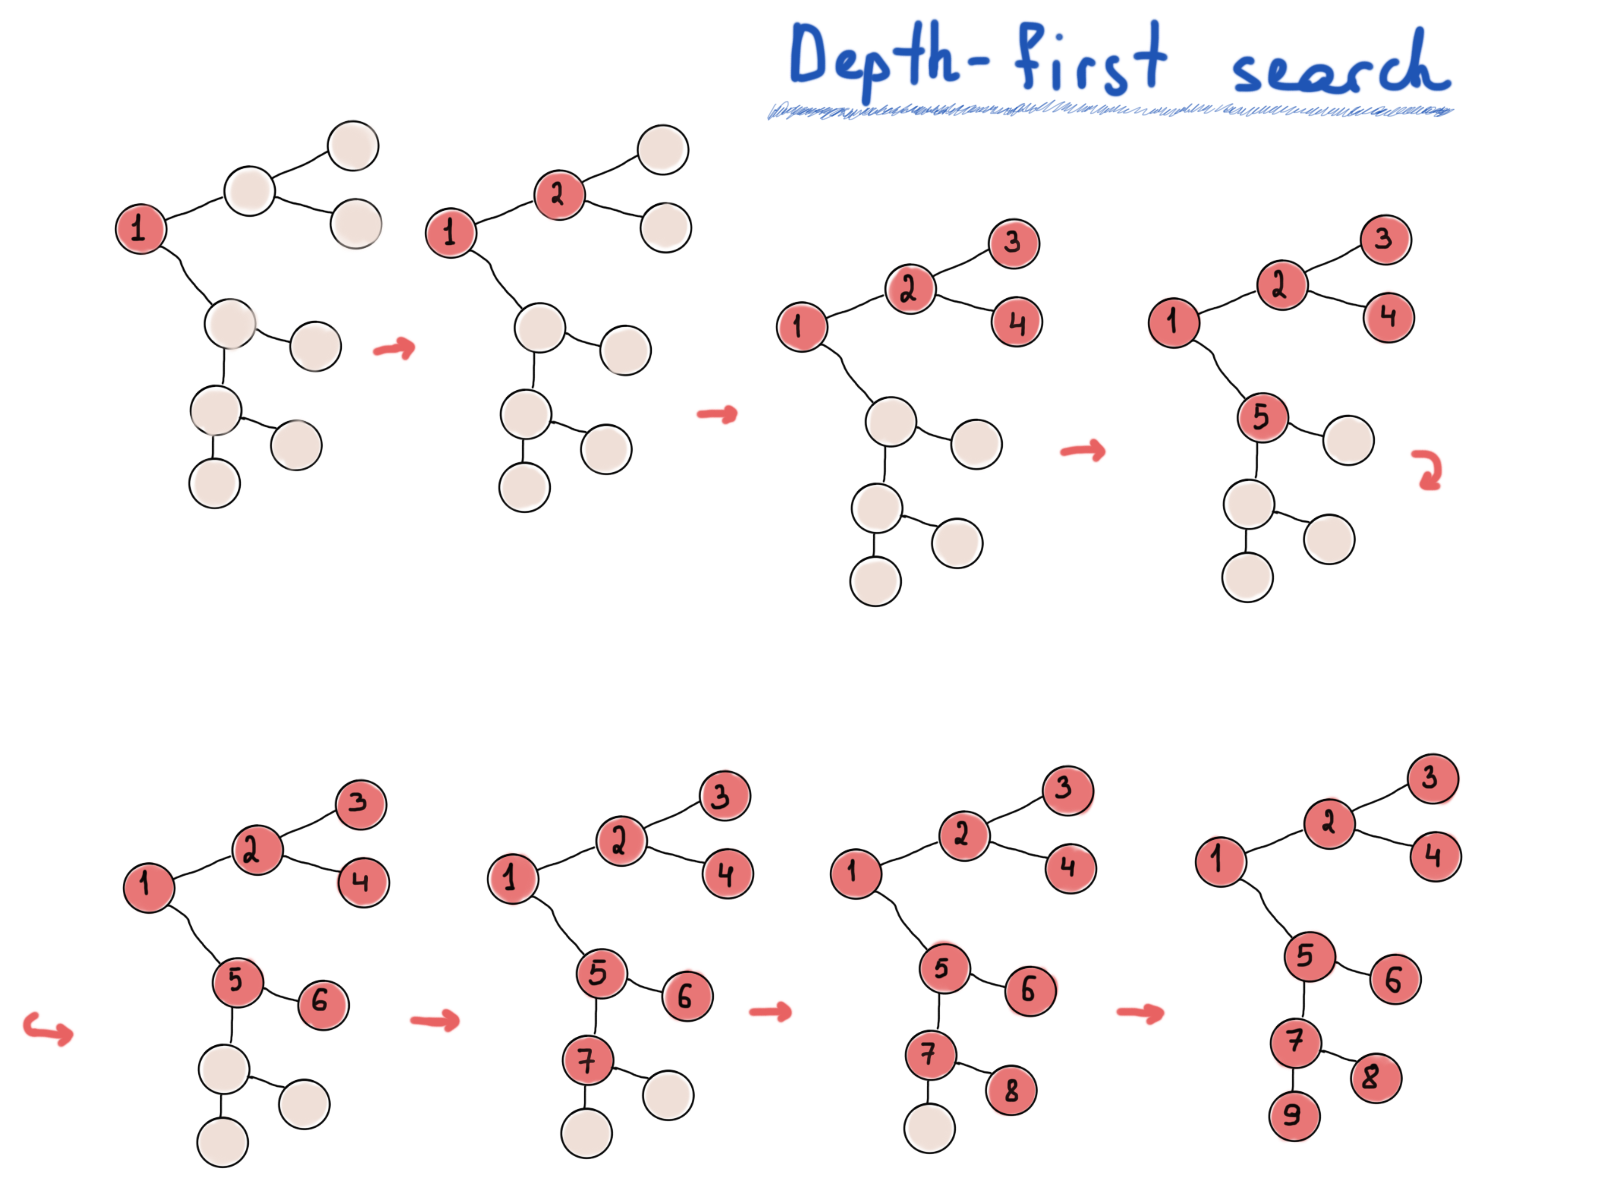
\includegraphics[width=10cm, height=7.7cm]{Term_2/Source/images/1_DFS.png}
\end{center}
\end{frame}

\begin{frame}[fragile]{Граф. Обход в глубину (DFS)}
\begin{center}
    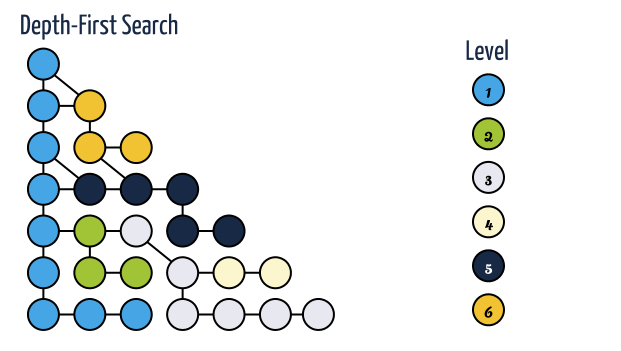
\includegraphics[width=10cm, height=5.7cm]{Term_2/Source/images/2_DFS_Graph.png}
\end{center}
\end{frame}

\begin{frame}[fragile]{Реализация обхода в глубину}
Как реализовать обход в глубину?
    \begin{itemize}
        \item В дереве - используем структуру дерева (у каждого узла известны дети). Делаем рекурсию в детей или через стэк.
        \item В графе - храним для каждой вершины маркер, заходили ли в него
\begin{lstlisting}
vector<bool> visited;
void dfs( int u ) {
    visited[u] = true;
    for( v: (u, v) ∈ E ) {
        if( !visited[v] ) {
            dfs( v );
        }
    }
}
int MainDFS() {
    visited.assign( n, false );
    for( int i = 0; i < n; ++i ) {
        if( !visited[i] ) {
            dfs( i );
        }
    }
}
\end{lstlisting}
    \end{itemize}
\end{frame}


\subsection{Поиск цикла}

\begin{frame}[fragile]{Поиск цикла}
Как найти цикл в графе?
    \begin{itemize}
        \item Если нашли ребро в уже посещенную вершину - значит, цикл есть.

    \end{itemize}
\end{frame}

\subsection{Топологическая сортировка}

\begin{frame}[fragile]{Ациклический ориентированный граф.}
Как обычно, в графе есть вершины, есть ребра. У каждого ребра есть направление.
\begin{center}
    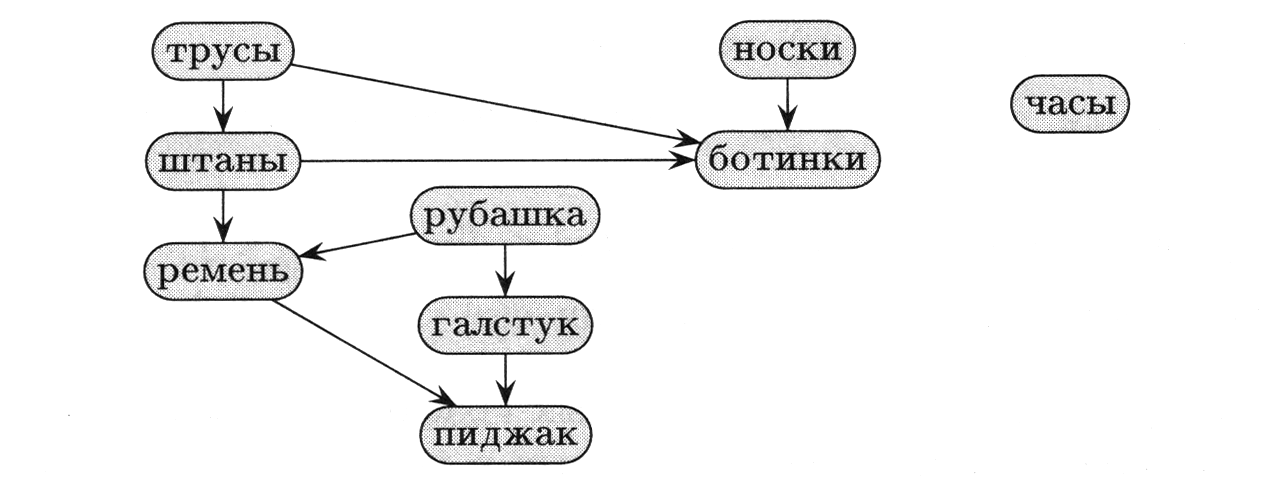
\includegraphics[width=10cm]{Term_2/Source/images/3_topological-sort-1.png}
\end{center}
\end{frame}

\begin{frame}[fragile]{Топологическая сортировка}

Граф иллюстрирует логический порядок надевания предметов одежды. Ребро от А к Б означает, что А следует надевать строго до Б. Отсутствие ребра означает, что порядок не важен.
\begin{center}
    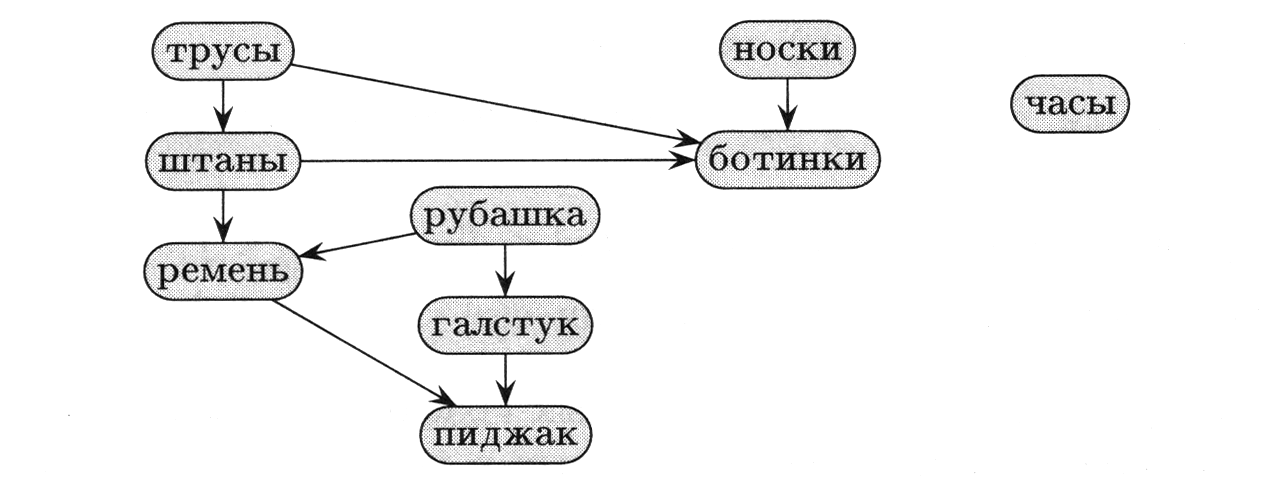
\includegraphics[width=10cm]{Term_2/Source/images/3_topological-sort-1.png}
\end{center}
\end{frame}


\begin{frame}[fragile]{Топологическая сортировка}
Задача.
В один момент времени вы можете надевать что-то одно. 

Нужно составить план надевания предметов, чтобы сохранить логические зависимости из графа (т.е. не надеть ботинки до носков)

Эта задача -- \textbf{топологическая сортировка}
\begin{center}
    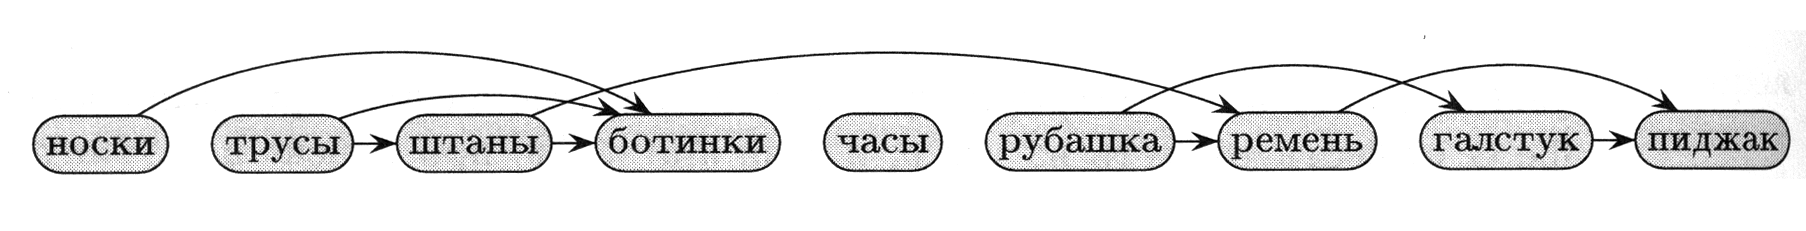
\includegraphics[width=10cm]{Term_2/Source/images/3_topological-sort-2.png}
\end{center}

\end{frame}

\begin{frame}[fragile]{Топологическая сортировка}

Как реализовать топологическую сортировку?
Внезапно нам поможет поиск в грубину с запоминанием времени входа и выхода из вершины.

    \begin{itemize}

        \item Создать пустой список вершин
        \item Вызвать DFS для каждой вершины
        \item В момент завершения обработки каждой вершины - добавить ее в начало списка.
        \item Вернуть полученный список
\end{itemize}

\end{frame}

\begin{frame}[fragile]{Топологическая сортировка}

Время входа и выхода из вершины обозначено слева от вершины: вход/выход.

\begin{center}
    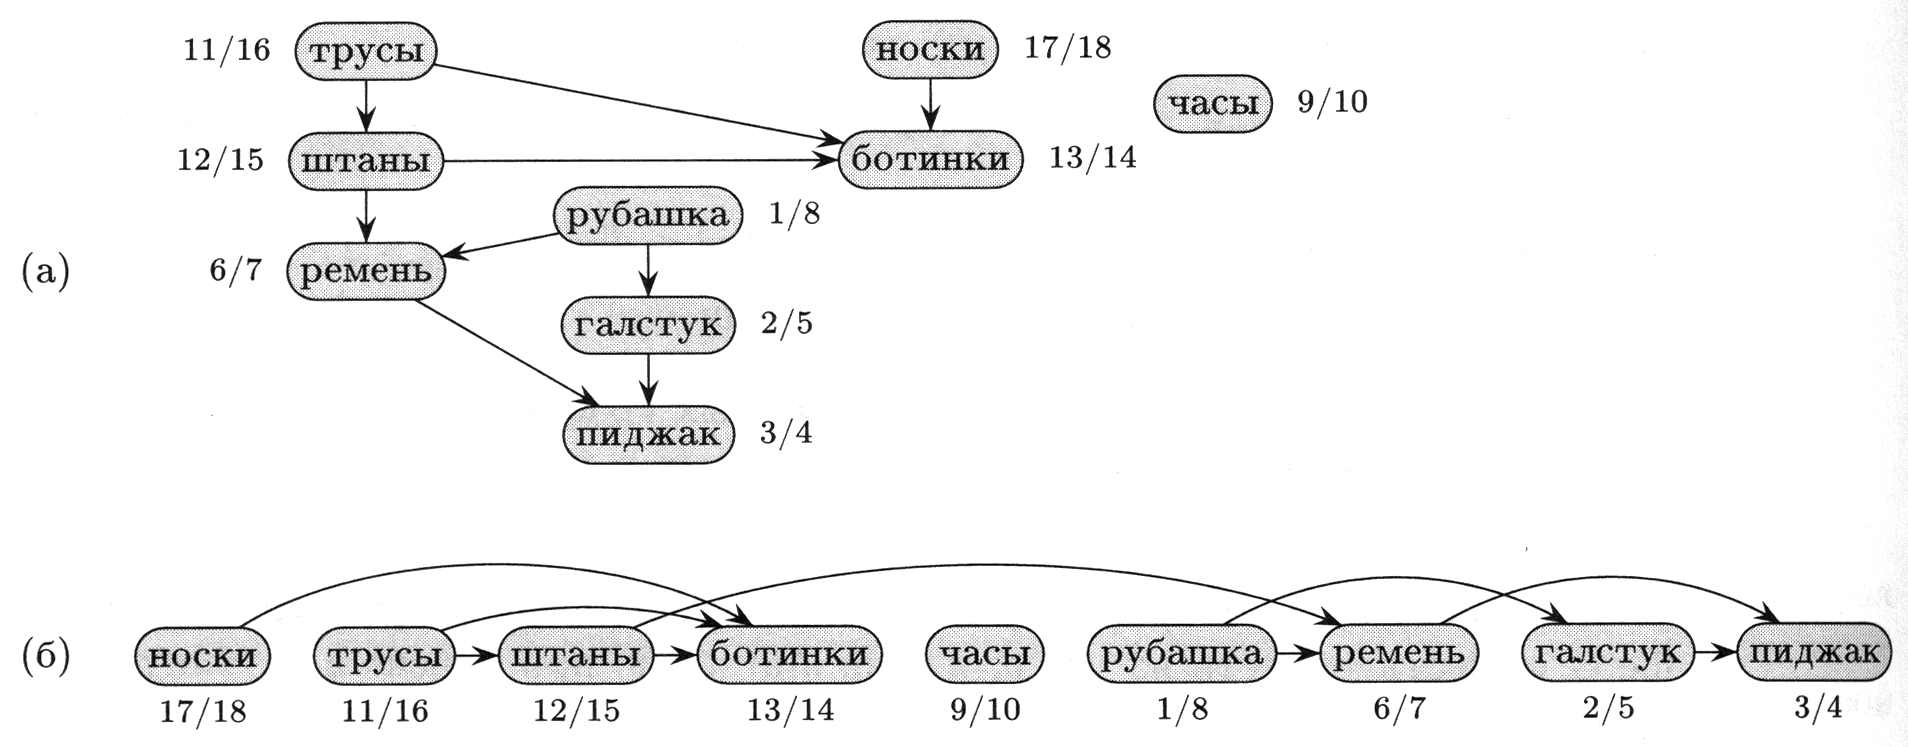
\includegraphics[width=10cm]{Term_2/Source/images/3_topological-sort.png}
\end{center}

\end{frame}

\appendix

\section<presentation>*{\appendixname}
\subsection<presentation>*{Useful links}

\end{document}


